\section{Further extensions}
\label{sec:futurework}

This section details further extensions on improving other aspects of the 
visualization system. For ideas on improving the specific work done in this 
thesis, see the extensions listed in Section~\ref{sec:al:extensions} for active 
learning, Section~\ref{sec:gc:extensions} for graph comparison, and 
Section~\ref{sec:usage:extensions} for portfolio management.

\subsection{Estimator selection}
\label{sec:futurework:estimatorselection}

Estimator selection involves actively fitting the ``best'' numerical model as 
opposed to passively
``checking'' a numerical model that's been given. For instance, rather than 
requiring a numerical model in order to compute the graph distance as in 
Chapter~\ref{ch:gc}, the VS would select a numerical model without requiring 
the analyst to fit one beforehand. This problem is more difficult
to solve in an objective manner, but such a function would be extremely useful 
in contributing to the idea of an accountable and reproducible ``clean 
analysis'' procedure.

\subsection{Outlier removal}
\label{sec:futurework:outlier}

Outliers are unavoidable in raw data and can skew results quite a bit. This can 
be seen in the analysis of Dataset 2 in Table~\ref{tab:intro:me} and 
Figure~\ref{fig:intro:meplot}. The question to answer here would be: when can 
the system remove outliers, and what criteria should it use to make this 
decision? The procedure should be both systematic and transparent so that the 
analyst and future readers may understand what has(n't) been removed and for 
what reason. Data given to the VS should be locked once analysis is complete so 
as to prevent analysts from maliciously removing or adding outliers themselves 
to favorably skew the results if the output is not to their liking, thereby 
increasing accountability. 

\subsection{Graphical models in finance}
\label{sec:futurework:graphicalmodel}

A single numerical correlation coefficient can be 
thought of as a regression of the response variable
against only one observed variable; it is a ``local'' property because it
compares the behavior of only two random variables. Correlations tend to fall 
short of the desired result due to the property of transitivity.

Transitivity states that if $X$ is correlated to $Y$, and $Y$ to $Z$,
then $X$ is also correlated to $Z$. Although correlation is not always
transitive, in situations where the correlations of various pairs are close to 
0 or 1, the data will often strongly exhibit properties of 
transitivity~\cite{tao2014}. Let us assume that the universe consists of Apple, 
Google, and Silicone (a manufacturer providing chips to both Apple and Google) 
stock. Suppose an analyst wants to model Google stock. 
Apple stock moves with Silicone stock as they
depend on them for their chips. Similarly, Google stock (unbeknownst to the
analyst) also moves with Silicone stock but not with Apple stock. Without 
considering the way the stocks are connected to the other observed variable 
(Silicone stock), it is simple to see how the correlation between observed 
prices of Google and Apple stock will be erroneously positive.

On the other hand, a single link in a graphical model can be thought of as a 
regression of the response variable against all variables in the space. The 
general idea is that a graphical model has a ``global'' property because it 
takes all other variables into account. Let $G=(V,E)$ be an undirected graph 
formed from the data set $X$ with $|V| =  n$ and edges $E_{i,j}\in\{0,1\}$. 
$E_{i,j}=1$ when there is an edge between $V_i$ and $V_j$, and 0 otherwise. 
$E_{i,j}=0$ if and only if $X_i \perp X_j$ given $X_k$ where $k\in\{1,...,d\}$ 
\textbackslash $\{i,j\}$. In other words, do not draw an edge if
$$\text{P}(X_i,X_j|X_k)=\text{P}(X_i|X_k)\text{P}(X_j|X_k)$$

The resulting graph is known as a graphical model. The drawback is the 
difficulty in empirically computing conditional distributions and the problems 
associated with fitting distributions to real data. 
However, the conditional independence of graphical models is more of a global 
property than correlation is because every pair of variables is conditioned on 
all other variables. Returning to the universe of Google, Apple, and Silicone 
stocks, conditioning Google on Silicone and Apple on Silicone would indicate 
that Google and Apple are uncorrelated. 

While correlation graphs and graphical models each have their own niche to 
fill, graphical model rebalancing has been shown to strongly outperform 
traditional portfolio management methods such as the ``buy and hold'' method 
employed in Chapter~\ref{ch:usage}~\cite{liuh2016}. 
It is important, therefore, for the VS to 
support both models. The system would need to be modified to allow for plotting 
$X_i$ against $X_j$ conditional on $X_k$ for all $k\in\{1,...,d\} \backslash 
\{i,j\}$. One method to consider would be to control for the behavior of all 
the other explanatory variables while making the pairwise scatter plot of 
$(X_i,X_j)$ in a procedure similar to that of regression.

\subsection{Ordering of queried plots}
\label{sec:futurework:ordering}

As people interact with graphs, they maintain a ``mental map'' of the 
graph; when users label a new graph, they remember the previous plots that they
have labeled~\cite{federico2016}. The importance of the mental map in 
influencing user perception of the data depends on
various factors such as the user preferences and tasks that they must
complete~\cite{federico2016}. Suppose that several active learning queries 
(pairwise scatter plots) are selected at once. Given a gradation of graphs 
(consecutive
graphs that are similar to one another), users are less able to 
distinguish differences than if they were given consecutive graphs from 
different 
ends of the spectrum~\cite{federico2016}. To put it 
concisely, the scatter plot display itself (discussed in 
Section~\ref{sec:visualizer:scatterplot:goodplot}) is not the only thing that 
matters. The ordering of the scatter plots also matter, and it is best to show 
the plots in an order that allows users to distinguish the differences among 
graphs that they have already seen. By improving user perception of the data, 
careful scatter plot ordering advances the accuracy of user responses. If user 
responses are to be thought of as observations of the user's true preferences, 
then the ordering of plots is another as a way to fine-tune the precision of 
the classifier. 

\subsection{Line-up tests}
\label{sec:futurework:lineup}

One of the pitfalls of data visualization is ``apophenia,'' a phenomenon where
the user sees patterns in random noise. Part of the reason this happens is due 
to the vagueness of defining ``independence'' on a non-uniform domain and range
(see Section~\ref{sec:visualizer:scatterplot:goodplot}). Wickham \textit{et 
al.} propose a line-up protocol that is similar to the Rorscach test (in which 
subjects are asked to interpret abstract blots of ink)~\cite{wickham2010}. 
In the line-up test, users are asked to identify the real data from a set of 
$k$ plots where $k-1$ plots are synthetically generated~\cite{wickham2010}.
Identification of the raw data against the synthetic data is an indicator 
that the current fitted model is a poor fit of the user's preferences. Suppose 
that $k = 5$ as in Figure~\ref{fig:visualizer:lineup}.
In the context of the classification problem, the line-up test may generate
four plots that are ``visually not correlated'' (following the proposed 
decision tree) 
and one plot that is ``visually correlated'' before asking the user if he/she 
can 
identify the ``visually correlated'' plot. If the user is able to consistently 
identify the ``visually correlated'' plot, it is an indication that the current 
decision tree is a close fit of the user's preferences.

\tablespacing
\begin{figure}[H]
	\begin{center}
		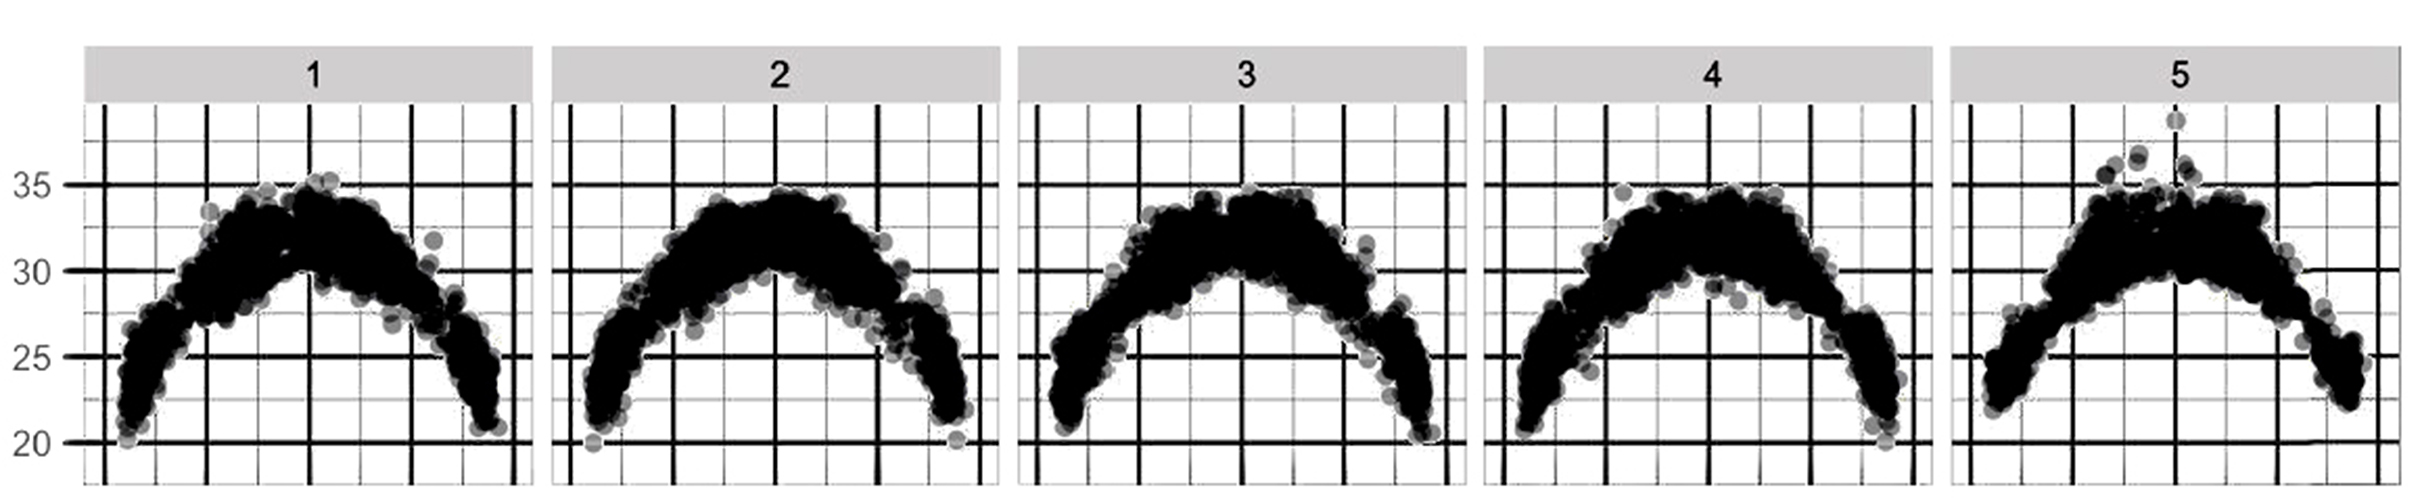
\includegraphics[width=1\linewidth]{ch-conclusion/figures/lineup}
		\caption[A line-up test for $k = 5$. ]{A line-up test for $k = 5$.
			Consistently identifying the raw data against the synthetic data 
			indicates that the fitted model may not be good enough. Figure from 
			Wickham \textit{et al.} 2010 with slight 
			modifications~\cite{wickham2010}}
		\label{fig:visualizer:lineup}
	\end{center}
\end{figure}
\bodyspacing

\subsection{Edge-weighted graphs}
\label{sec:futurework:edgeweighted}

Edge-weighted graphs stray from the binary classification of 
correlation graphs (described in Section~\ref{sec:intro:correlation}) and 
graphical models (described in Section~\ref{sec:futurework:graphicalmodel}). In 
an edge-weighted graph, edges are weighted depending
on the type of conditional dependence (e.g. correlation). Negative and positive 
values are assigned 1 and -1, respectively. As before, a value of 0 (no edge) 
implies that variables are uncorrelated (for correlation graphs) or 
conditionally independent (for graphical models). Active learning becomes 
more difficult as the number of classification labels changes from two to 
three. Subsequently, active learning methods may need to be more generalized as 
in the case of uncertainty sampling (Section~\ref{sec:al:methods:uncertainty}). 

\subsection{Rejection classification}
\label{sec:futurework:rejection}

While interacting with the data visually, the user's own concept of ``visual 
correlation'' \textit{in the specific data set} may evolve over time; at the 
beginning, the user has no idea what the data looks like and where to set the 
bar for their own standards of dependence. There are several 
ways to take this into consideration. 

\tablespacing
\begin{itemize}
	\item The visualization system could assign a weight to the analyst's 
	responses by trial number where the last few plots are more valuable than 
	the first few. However, this may destabilize cases where the user's 
	preferences don't end up changing.
	
	\item The system can include an alternative option that allows the user to 
	refuse to label a plot when it's too close to their decision boundary. This 
	is welcome for the user who is not forced into making a decision he/she is 
	uncertain about, but it is problematic for the learner as it causes the 
	hypothesis space to remain unchanged rather than shrink. The point of the 
	active learning in stage 1 (Section~\ref{sec:visualizer:al}, 
	Chapter~\ref{ch:al}) is to have the user provide labels on plots the 
	learner is uncertain about in order to 
	better understand user preferences. By allowing for this option, the active
	learner may require more queries and/or return a poorly-defined forest. 
	
	\item Aside from the current responses of ``yes, visually correlated'' and 
	``no, visually not correlated'', the VS could 
	include a third option that permits the user to ``recycle'' the plot. This 
	method allows the user to return to the plot later after learning more 
	about what the rest of the data looks like and understanding his/her own 
	preferences better, and it also ensures that the active learner will 
	eventually receive a label for all its queries. This method could 
	potentially de-balance an ordering procedure (described in 
	Section~\ref{sec:futurework:ordering}), but the VS can strategically 
	account for both by inserting the recycled plot between two plots it is 
	relatively different from with the constraint that the insertion location 
	is after the current plot.
\end{itemize}
\bodyspacing
